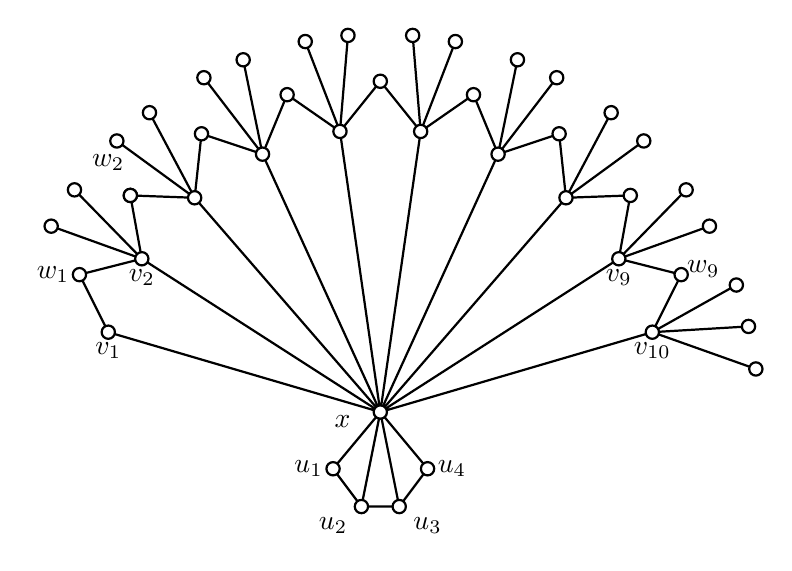
\begin{tikzpicture}[scale=1.2,style=thick]
  \def\vr{2pt} % \vr = vertex radius;  Set \vr = 2/scale for uniform sizing
  of vertices
  %%% define points
  \path (0,0) coordinate (x);
  %%%


  \path (x) +(-180-180/11:3) coordinate (v1);
  \path (x) +(-180-180*2/11:3) coordinate (v2);
  \path (x) +(-180-180*3/11:3) coordinate (v3);
  \path (x) +(-180-180*4/11:3) coordinate (v4);
  \path (x) +(-180-180*5/11:3) coordinate (v5);
  \path (x) +(-180-180*6/11:3) coordinate (v6);
  \path (x) +(-180-180*7/11:3) coordinate (v7);
  \path (x) +(-180-180*8/11:3) coordinate (v8);
  \path (x) +(-180-180*9/11:3) coordinate (v9);
  \path (x) +(-180-180*10/11:3) coordinate (v10);
  %%%
  \path (x) +(-180-180*1.5/11:3.5) coordinate (w1);
  \path (x) +(-180-180*2.5/11:3.5) coordinate (w2);
  \path (x) +(-180-180*3.5/11:3.5) coordinate (w3);
  \path (x) +(-180-180*4.5/11:3.5) coordinate (w4);
  \path (x) +(-180-180*5.5/11:3.5) coordinate (w5);
  \path (x) +(-180-180*6.5/11:3.5) coordinate (w6);
  \path (x) +(-180-180*7.5/11:3.5) coordinate (w7);
  \path (x) +(-180-180*8.5/11:3.5) coordinate (w8);
  \path (x) +(-180-180*9.5/11:3.5) coordinate (w9);
  %%%
  \path (x) +(-180-180*1.8/11:4) coordinate (a2);
  \path (x) +(-180-180*2.2/11:4) coordinate (b2);
  \path (x) +(-180-180*2.8/11:4) coordinate (a3);
  \path (x) +(-180-180*3.2/11:4) coordinate (b3);
  \path (x) +(-180-180*3.8/11:4) coordinate (a4);
  \path (x) +(-180-180*4.2/11:4) coordinate (b4);
  \path (x) +(-180-180*4.8/11:4) coordinate (a5);
  \path (x) +(-180-180*5.2/11:4) coordinate (b5);
  \path (x) +(-180-180*5.8/11:4) coordinate (a6);
  \path (x) +(-180-180*6.2/11:4) coordinate (b6);
  \path (x) +(-180-180*6.8/11:4) coordinate (a7);
  \path (x) +(-180-180*7.2/11:4) coordinate (b7);
  \path (x) +(-180-180*7.8/11:4) coordinate (a8);
  \path (x) +(-180-180*8.2/11:4) coordinate (b8);
  \path (x) +(-180-180*8.8/11:4) coordinate (a9);
  \path (x) +(-180-180*9.2/11:4) coordinate (b9);
  \path (x) +(-180-180*9.8/11:4) coordinate (a10);
  \path (x) +(-180-180*10.2/11:4) coordinate (b10);
  \path (x) +(-180-180*10.6/11:4) coordinate (c10);
  %%% body of the peacock
  \path (-0.5,-0.6) coordinate (leg1);
  \path (-0.2,-1) coordinate (leg2);
  \path (0.2,-1) coordinate (leg3);
  \path (0.5,-0.6) coordinate (leg4);
  %%% Edges:
  \draw (v1) -- (x) -- (v2);
  \draw (v3) -- (x) -- (v4);
  \draw (v5) -- (x) -- (v6);
  \draw (v7) -- (x) -- (v8);
  \draw (v9) -- (x) -- (v10);
  %%%
  \draw (v1) -- (w1) -- (v2) -- (w2) -- (v3) -- (w3) -- (v4) -- (w4) -- (v5) -- (w5) -- (v6) -- (w6) -- (v7) -- (w7) -- (v8) -- (w8) -- (v9) -- (w9) -- (v10);
  %%%
  \draw (a2) -- (v2) -- (b2);
  \draw (a3) -- (v3) -- (b3);
  \draw (a4) -- (v4) -- (b4);
  \draw (a5) -- (v5) -- (b5);
  \draw (a6) -- (v6) -- (b6);
  \draw (a7) -- (v7) -- (b7);
  \draw (a8) -- (v8) -- (b8);
  \draw (a9) -- (v9) -- (b9);
  \draw (a10) -- (v10) -- (b10);
  \draw (v10) -- (c10);
  %%%
  \draw (leg1) -- (leg2) -- (leg3) -- (leg4);
  \draw (leg1) -- (x) -- (leg2);
  \draw (leg3) -- (x) -- (leg4);
  %%% Vertices:
  \draw (x) [fill=white] circle (\vr);
  \draw (v1) [fill=white] circle (\vr); \draw (v2) [fill=white] circle (\vr);
  \draw (v3) [fill=white] circle (\vr); \draw (v4) [fill=white] circle (\vr);
  \draw (v5) [fill=white] circle (\vr); \draw (v6) [fill=white] circle (\vr);
  \draw (v7) [fill=white] circle (\vr); \draw (v8) [fill=white] circle (\vr);
  \draw (v9) [fill=white] circle (\vr); \draw (v10) [fill=white] circle (\vr);
  %%%
  \draw (w1) [fill=white] circle (\vr); \draw (w2) [fill=white] circle (\vr);
  \draw (w2) [fill=white] circle (\vr); \draw (w3) [fill=white] circle (\vr);
  \draw (w4) [fill=white] circle (\vr); \draw (w5) [fill=white] circle (\vr);
  \draw (w6) [fill=white] circle (\vr); \draw (w7) [fill=white] circle (\vr);
  \draw (w8) [fill=white] circle (\vr); \draw (w9) [fill=white] circle (\vr);
  %%%
  \draw (a2) [fill=white] circle (\vr); \draw (b2) [fill=white] circle (\vr);
  \draw (a3) [fill=white] circle (\vr); \draw (b3) [fill=white] circle (\vr);
  \draw (a4) [fill=white] circle (\vr); \draw (b4) [fill=white] circle (\vr);
  \draw (a5) [fill=white] circle (\vr); \draw (b5) [fill=white] circle (\vr);
  \draw (a6) [fill=white] circle (\vr); \draw (b6) [fill=white] circle (\vr);
  \draw (a7) [fill=white] circle (\vr); \draw (b7) [fill=white] circle (\vr);
  \draw (a8) [fill=white] circle (\vr); \draw (b8) [fill=white] circle (\vr);
  \draw (a9) [fill=white] circle (\vr); \draw (b9) [fill=white] circle (\vr);
  \draw (a10) [fill=white] circle (\vr); \draw (b10) [fill=white] circle (\vr);
  \draw (c10) [fill=white] circle (\vr);
  %%% 
  \draw (leg1) [fill=white] circle (\vr);
  \draw (leg2) [fill=white] circle (\vr);
  \draw (leg3) [fill=white] circle (\vr);
  \draw (leg4) [fill=white] circle (\vr);
  %%% text
  \draw (-0.4,-0.1) node {$x$};
  \draw [below] (v1) node {$v_1$};
  \draw [below] (v2) node {$v_2$};
  \draw [below] (v9) node {$v_9$};
  \draw [below] (v10) node {$v_{10}$};
  \draw [left] (w1) node {$w_1$};
  \draw (w2) node[xshift=-8pt, yshift=12pt] {$w_2$};
  \draw (w9) node[xshift=8pt, yshift=2pt] {$w_9$};
  \draw [left] (leg1) node {$u_1$};
  \draw (-0.5,-1.2) node {$u_2$};
  \draw (0.5,-1.2) node {$u_3$};
  \draw [right] (leg4) node {$u_4$};
\end{tikzpicture}
